\documentclass[11pt,a4paper]{article}
\usepackage[margin=20mm]{geometry}
\usepackage[T1]{fontenc}
\usepackage{graphicx}
\usepackage{longtable}
\usepackage{array}
\usepackage{fancyvrb}
\usepackage{hyperref}
\hypersetup{colorlinks=true,linkcolor=black,urlcolor=black}
\setlength{\parskip}{0.35em}
\begin{document}
\begin{titlepage}
\vspace*{25mm}
\begin{center}

\includegraphics[width=0.56\linewidth]{assets/cover_logo_1.png}\hfill
\includegraphics[width=0.24\linewidth]{assets/cover_logo_2.png}\\[3mm]
\hfill{\bfseries Forgebots}\\[35mm]
\rule{\linewidth}{0.7pt}\\[15mm]
{\Huge\bfseries Teaching a Giant Airliner to Take Off}\\[12mm]
{\Large A from-zero guide to reinforcement learning, this project, and rebuilding it step by step}\\[16mm]
\rule{\linewidth}{0.7pt}\\[35mm]
{\large Project handbook: 8 October 2026}
\end{center}
\end{titlepage}
\begin{abstract}
One sentence: A simulated pilot learns to control throttle, elevator, aileron and rudder so a research approximation of a Boeing 747-8 can perform a clean, stable takeoff in changing conditions.
\end{abstract}
\begin{figure}[htbp]\centering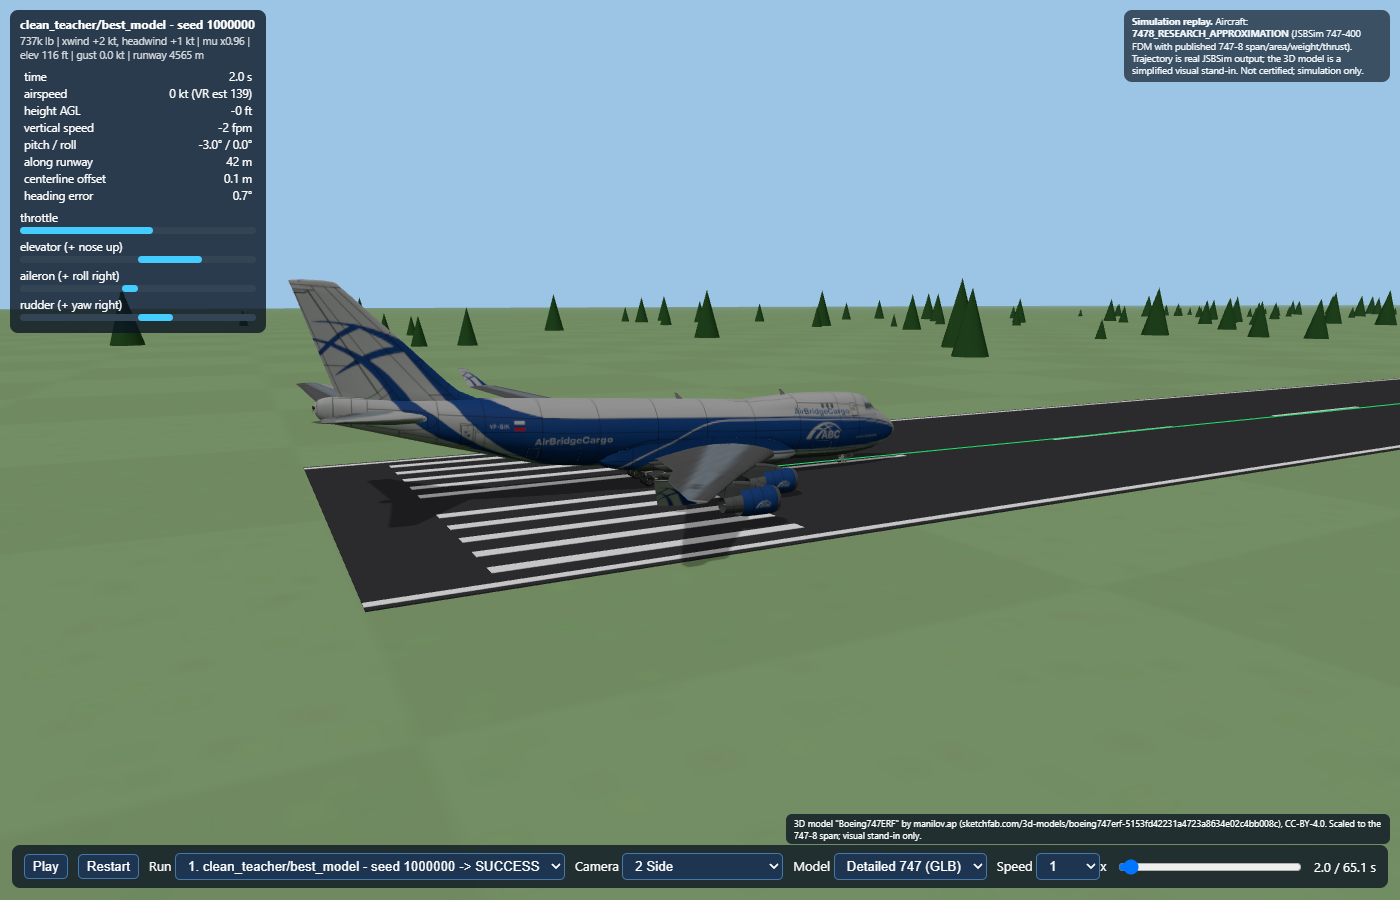
\includegraphics[width=0.9\linewidth]{../assets/simulation_3d.png}\caption{The project replay viewer. The displayed aircraft does not supply the flight physics; JSBSim does.}\end{figure}
\section*{How to use this report}
Read sections 1-5 for the basic idea, 6-14 for the exact implementation, 15 for visual evidence, and 16-22 when you want to rebuild or continue the work. No machine-learning background is required.
\clearpage
\tableofcontents
\clearpage
\section{The whole story in two minutes}
Imagine teaching someone to take off in a simulator. You put the airplane at the start of a runway, let the student move four controls, tell them what happened, and repeat. The student is a computer program called an agent. The simulator is JSBSim. The teacher is optional example code. The score is a reward. The final exam uses runway and weather conditions that the training run did not memorize.

\begin{figure}[htbp]\centering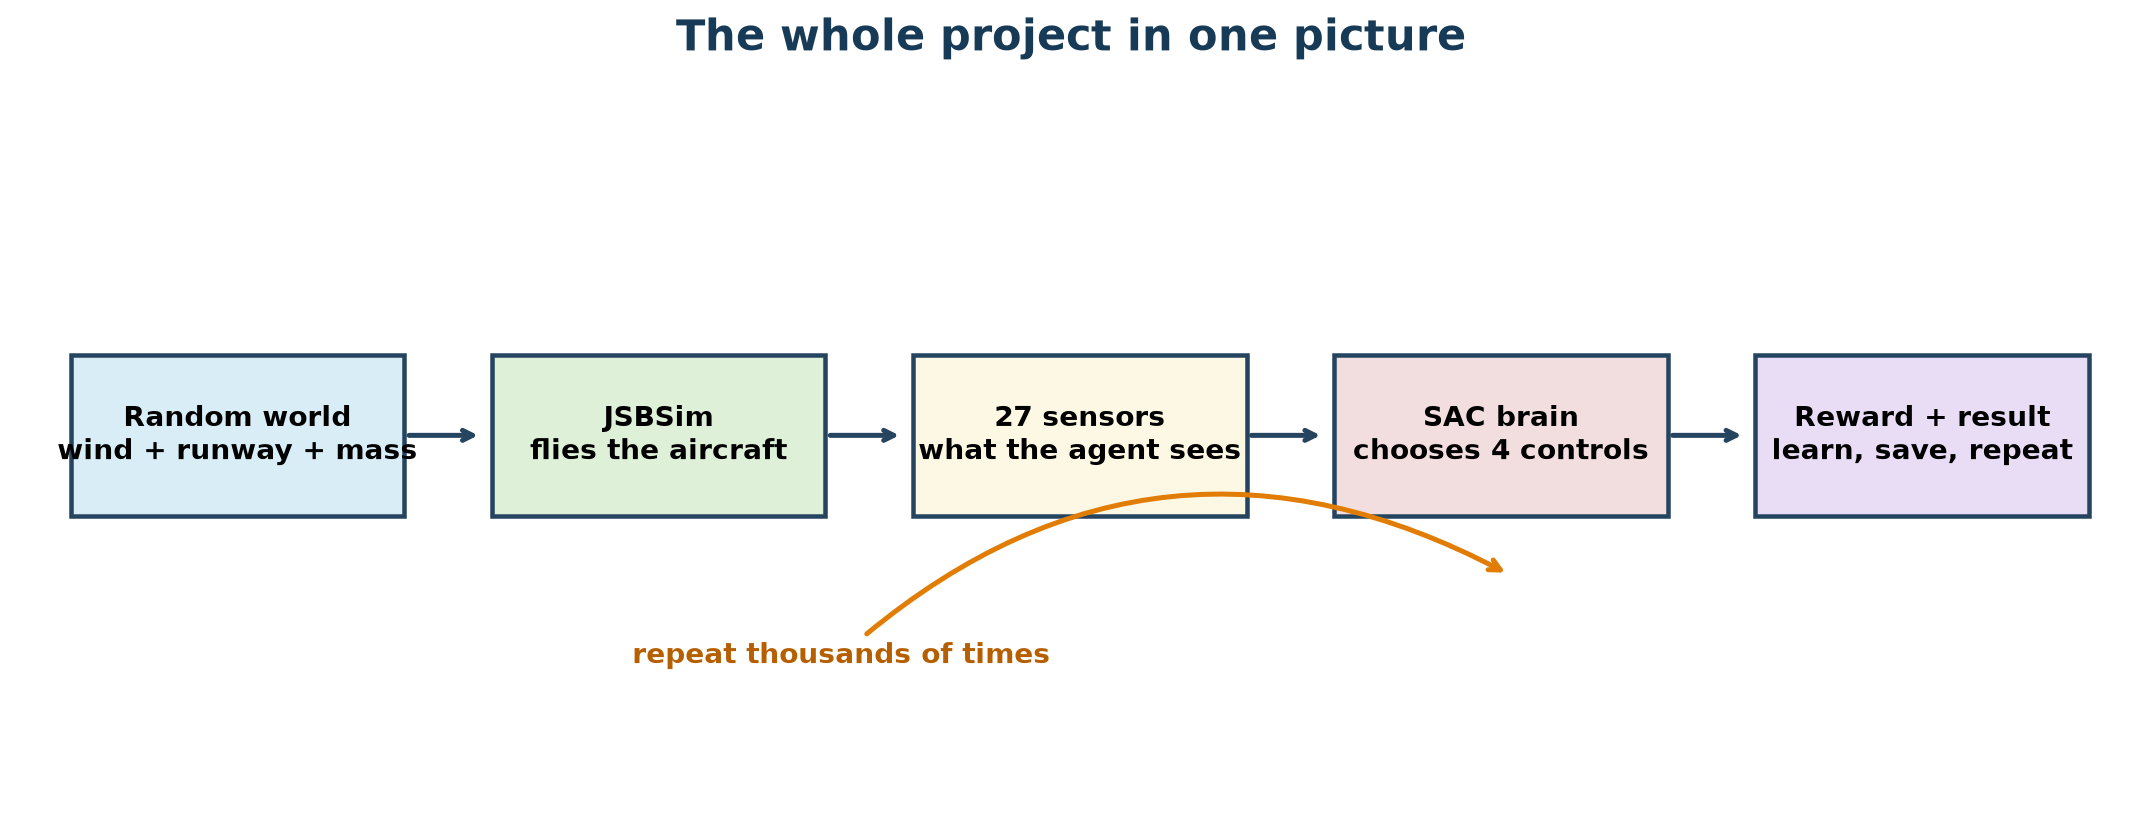
\includegraphics[width=0.96\linewidth]{../assets/project_flow.png}\caption{The project loop: conditions -> simulator -> observations -> agent -> controls -> new simulator state -> reward.}\end{figure}
One attempt is an episode. An episode begins with engines running, flaps set and gear down. It ends in a stable success, a named failure, or a time limit. The agent only chooses throttle, elevator, aileron and rudder; it does not configure flaps, gear, brakes or trim during an episode.

\begin{longtable}{|p{0.313\linewidth}|p{0.313\linewidth}|p{0.313\linewidth}|}\hline
Everyday idea & Project name & Why it exists \\ \hline
Student & agent / policy & Chooses the next control action. \\ \hline
Practice room & environment & Runs physics and returns feedback. \\ \hline
What the student sees & observation & 27 measured or derived numbers. \\ \hline
What the student does & action & Four requested control values. \\ \hline
Score & reward & Small clues plus a large valid-success bonus. \\ \hline
One try & episode & A full runway-to-outcome attempt. \\ \hline
Harder lessons & curriculum & Expands weather, weight and runway difficulty. \\ \hline
\end{longtable}
\section{Before machine learning: what is a takeoff?}
The airplane must accelerate along the runway while staying near its center line. Near an estimated rotation speed, it raises its nose smoothly. It lifts off, climbs, reaches 1,000 feet above the runway, and stays within the allowed speed and attitude limits for five seconds. A rough or wandering path can still fail the cleanliness rule.

\begin{figure}[htbp]\centering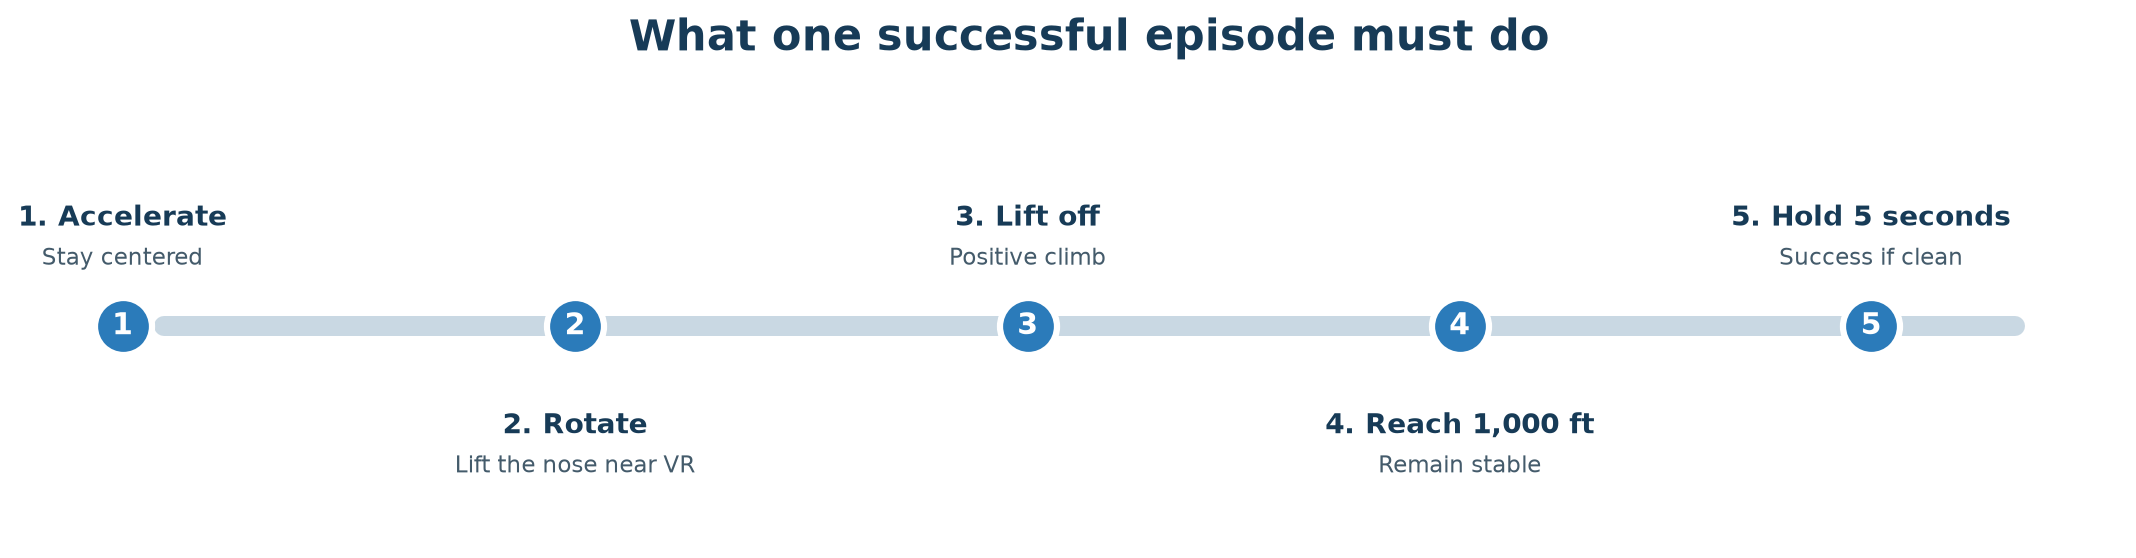
\includegraphics[width=0.96\linewidth]{../assets/takeoff_story.png}\caption{The takeoff as a story: roll, steer, rotate, lift off, climb, stabilize.}\end{figure}
Airspeed is motion relative to the air; ground speed is motion over the runway. In a headwind they differ. Pitch is nose up or down. Roll is wing tilt. Heading is where the nose points. Course is where the airplane actually moves. Centerline error is sideways distance from the runway middle. AGL means height above the local ground reference. The code uses meters for runway position, knots for airspeed, feet for height, and feet per minute for climb rate; conversions happen before values enter the policy.

\section{Reinforcement learning without jargon}
Ordinary supervised learning says, 'Here is the right answer for this example.' Reinforcement learning says, 'Try an action; here is what happened and how useful it was.' The agent must discover a sequence of actions whose total score is high. A takeoff is a sequence problem: a good throttle choice now changes the speed available for rotation later.

At time t, the observation is s(t), the action is a(t), the reward is r(t), and the next observation is s(t+1). The policy is a function that maps s(t) to a(t). Its goal is to maximize the expected sum of future rewards, often written r(0) + gamma r(1) + gamma squared r(2) + ... . Gamma, set to 0.995 here, makes near-future and later consequences matter.

Tiny example: a sharp rudder movement might give an immediate centerline improvement, but it can cause a later swing. The agent should value the whole flight, not only the next tenth of a second.

Exploration means trying uncertain actions during training. Evaluation turns that randomness off so repeated exams are comparable. A replay buffer is a notebook of past (observation, action, reward, next observation, done) transitions. The agent samples old notebook entries to learn without repeating every flight immediately.

\section{Why SAC, neural networks and a teacher?}
The four controls are continuous values between -1 and 1. Soft Actor-Critic (SAC) is designed for continuous actions. A DQN-style menu of discrete actions would need an artificial grid of control positions. The SAC actor is a neural network that proposes actions. Two critic networks estimate how valuable actions are; using two helps limit overly optimistic estimates. 'Soft' means the objective also rewards enough exploration, controlled by an automatically adjusted entropy coefficient.

A neural network here is a set of adjustable numbers. Three hidden layers with 256 units each give the actor and critics enough flexibility to connect speed, wind, runway error and control choices. ReLU is the activation function. Backpropagation adjusts the network weights after sampling experiences from the replay buffer. The learning rate, 0.0003, controls the size of those adjustments.

The teacher is a plain feedback controller. It gives full thrust, steers toward the runway center, waits for an estimated rotation speed and then targets a climb pitch. Its demonstrations can fill the replay buffer, and behavior cloning can teach the actor to imitate example actions before SAC exploration. The teacher is a learning aid and a debugging baseline, not a certified flight controller.

\begin{longtable}{|p{0.313\linewidth}|p{0.313\linewidth}|p{0.313\linewidth}|}\hline
Setting in configs/sac.yaml & Value & Plain purpose \\ \hline
buffer\_size & 1,000,000 & How many past transitions the notebook can hold. \\ \hline
learning\_starts & 10,000 & Gather experience before regular gradient updates. \\ \hline
batch\_size & 256 & Past transitions sampled for one update. \\ \hline
gamma & 0.995 & How much later rewards count. \\ \hline
tau & 0.005 & How slowly target critics follow learned critics. \\ \hline
train\_freq / gradient\_steps & 1 / 1 & One learning update per new transition. \\ \hline
ent\_coef & auto & Let SAC tune exploration pressure. \\ \hline
\end{longtable}
\section{One episode, viewed as a flowchart}
First, reset chooses an episode seed and difficulty, samples aircraft loading, runway and weather, and initializes the simulator. Then the program reads sensors and converts them to a 27-number observation. The agent chooses four controls. An actuator mapper limits how fast each control may move. JSBSim runs 12 small physics steps while that command is held. The program reads the new state, checks success and failure, computes reward and sends the new observation back. The cycle repeats at 10 actions per simulated second.

\begin{longtable}{|p{0.313\linewidth}|p{0.313\linewidth}|p{0.313\linewidth}|}\hline
Stage & Code owner & What to inspect when it fails \\ \hline
Load YAML & envs/\_\_init\_\_.py & Wrong config directory or missing key. \\ \hline
Build aircraft & envs/jsbsim\_interface.py & XML generation, properties, model status. \\ \hline
Draw conditions & envs/randomization.py & Difficulty level, seed, ranges. \\ \hline
Run physics & envs/jsbsim\_interface.py & JSBSim property values and non-finite state. \\ \hline
Build observations & envs/observations.py & Order, units, scaling, clipping. \\ \hline
Apply actions & envs/actions.py & Signs, limits, throttle mapping. \\ \hline
Decide outcome & envs/termination.py & Success hold, failure priority, timeout. \\ \hline
Score flight & envs/reward.py & Each reward component and profile. \\ \hline
Train / save & training/train\_sac.py & SAC, teacher data, resume, callbacks. \\ \hline
\end{longtable}
\section{What the agent sees: all 27 observations}
The policy cannot look at the 3D picture. It receives a fixed list of numbers, always in the order below. The order is part of the interface: changing it without updating a saved policy breaks that policy. Values are divided by a configured scale and clipped to -5 through 5 so very large numbers do not overwhelm the neural network. A non-finite value is treated as a simulator error.

\begin{longtable}{|p{0.313\linewidth}|p{0.313\linewidth}|p{0.313\linewidth}|}\hline
Number & Names & Meaning and reason \\ \hline
1-4 & airspeed, ground\_speed, agl, vertical\_speed & Know whether to accelerate, rotate and climb. \\ \hline
5-8 & pitch, roll, relative\_heading, alpha & Know attitude and whether the wing is near a dangerous angle. \\ \hline
9-12 & beta, p, q, r & Know side slip and how fast the aircraft rotates. \\ \hline
13-16 & lateral\_error, course\_error, distance\_travelled, distance\_remaining & Stay centered and know runway left. \\ \hline
17-21 & weight\_on\_wheels, elevator\_pos, aileron\_pos, rudder\_pos, throttle & Know airborne/ground state and actual actuator positions. \\ \hline
22-24 & engine\_n1, mass\_norm, cg\_norm & Know engine response and loading. \\ \hline
25-27 & headwind, crosswind, density\_ratio & Adapt to weather and thinner air. \\ \hline
\end{longtable}
Example: if the airplane is 6 meters right of center and the scale is 30 meters, the lateral input is 6/30 = 0.2. The positive sign means right. The teacher interprets this and commands a small leftward heading. 'Normalized' means made comparable in size; it does not mean the physical quantity disappears.

\section{What the agent does: four requested actions}
The agent outputs [throttle, elevator, aileron, rudder], each in [-1, 1]. Throttle -1 means idle and +1 means full lever; the other three use +elevator for nose up, +aileron for roll right and +rudder for yaw right. JSBSim uses different signs for some axes, so the mapper changes signs before sending commands. Nose-wheel steering follows rudder on the ground. Each actuator moves toward the request at a limited rate, rather than jumping instantly.

\begin{longtable}{|p{0.235\linewidth}|p{0.235\linewidth}|p{0.235\linewidth}|p{0.235\linewidth}|}\hline
Action & Sign sent to JSBSim & Rate limit per second & Why this matters \\ \hline
Throttle & Mapped from [-1,1] to [0,1] & 0.5 & Avoid instant engine-lever jumps. \\ \hline
Elevator & -1 & 1.0 & Make agent-positive mean nose up. \\ \hline
Aileron & +1 & 1.5 & Make agent-positive mean right roll. \\ \hline
Rudder & -1; steering +1 & 1.5 & Make agent-positive mean right yaw and wheel turn. \\ \hline
\end{longtable}
The action mapper checks shape and rejects NaN or infinity. It clips commands to the allowed range, maps throttle, computes the difference from the current actuator position, clips that difference by rate times 0.1 second, and only then sends JSBSim commands. This is why the policy observes actuator positions: the requested control and the actual control may temporarily differ.

\section{The airplane model: what is real and what is assumed}
JSBSim is the physics calculator. It is not the 3D viewer. The repository found no validated JSBSim 747-8 flight-dynamics model. It starts from JSBSim's community Boeing 747-400 model and changes a short list of public 747-8 figures: wingspan, wing area, empty weight, fuel capacity and engine thrust. Aerodynamic tables, inertia, landing gear and many engine details remain from the 747-400. The generated aircraft is explicitly named 7478\_RESEARCH\_APPROXIMATION.

A picture of a 747 in the replay can be visually convincing while the underlying physics remains approximate. The 3D mesh is a display stand-in and never supplies lift or thrust to JSBSim. Therefore, every performance result here is a result about this simulator setup, not a real 747-8.

The model also estimates rotation speed from a simplified stall-speed formula. This helps the agent and teacher know roughly when rotation is plausible; it is not a Boeing takeoff chart. Fuel is placed at the center of gravity in the approximation, runway slope is unsupported, tire friction uses multipliers, and some limits are engineering choices. For a more faithful study, a validated aircraft model and real performance comparisons are essential.

\section{Randomization: the practice room changes}
If every practice flight had the same weight, wind and runway, the agent could memorize one trick. The randomizer changes mass, center of gravity, runway length/elevation/friction/heading, temperature, pressure, wind, gusts, turbulence and small starting errors. A fixed seed reproduces the same draw, which is valuable for debugging.

The curriculum begins with level 1: easy but still variable. Levels 2, 3 and 4 widen the conditions. Level 5 in this repository explores very slippery runway cases. Twenty percent of training episodes can be drawn from a lower level, so the policy keeps practicing old skills. The promotion rule uses deterministic evaluation on at least 20 episodes and requires success strictly above 80 percent.

\begin{longtable}{|p{0.313\linewidth}|p{0.313\linewidth}|p{0.313\linewidth}|}\hline
Level & Plain interpretation & Example challenge \\ \hline
1 & Learn the basic roll and climb & Light wind, long runway, moderate mass. \\ \hline
2 & Add noticeable variation & More crosswind, CG shift and runway drag. \\ \hline
3 & Intended broad training & Heavier mass, stronger wind, shorter runway. \\ \hline
4 & Robustness stress & Wider weather and runway ranges. \\ \hline
5 & Slippery-runway curiosity & Very low tire-friction factors. \\ \hline
\end{longtable}
\section{Reward: the coach's point system}
The final success rule is the goal. Dense reward gives useful clues along the way so the agent can learn before its first full takeoff. A small positive score encourages forward progress, correct heading, centerline tracking, acceleration, controlled rotation, climb and time spent stable. Penalties discourage sideways drift, large roll or heading error, excessive angle of attack, sideslip, fast control changes, early rotation and named failures.

The clean profile adds a tighter centerline reward and penalties for sideways speed/acceleration and rocking. At a valid takeoff it pays a bonus proportional to whole-flight cleanliness. The baseline profile zeros those comfort terms for comparison. Changing reward profiles changes the task; resume a checkpoint only with its original profile unless deliberately starting a new experiment.

\begin{longtable}{|p{0.47\linewidth}|p{0.47\linewidth}|}\hline
Question & Answer \\ \hline
Why reward progress? & A full takeoff can be rare at first; progress gives an early learning signal. \\ \hline
Why a large success bonus? & The complete stable takeoff must matter more than farming small step rewards. \\ \hline
Why a small time penalty? & We want timely takeoff only after safe completion, not speed at any cost. \\ \hline
Why speed-gate alignment reward? & Otherwise the policy could earn centerline points while standing still. \\ \hline
Why cap squared penalties? & A single extreme state should not create an unstable giant training signal. \\ \hline
Why separate components? & The training CSV can reveal which behavior is rewarded or punished. \\ \hline
\end{longtable}
A useful debugging example: if the plane accelerates but swerves, inspect centerline reward, lateral penalty, heading penalty and control-oscillation penalty in the episode CSV. Do not change five weights at once; change one hypothesis, run the same evaluation seeds, and compare against the prior result.

\section{Success, failure and timeouts}
Success is deliberately harder than 'the wheels left the ground.' The aircraft must be airborne, reach 1,000 ft AGL, climb at least 500 ft/min, stay within roll/pitch/heading/angle-of-attack/sideslip/centerline limits, and maintain enough airspeed. These conditions must hold for 50 consecutive 0.1-second policy steps. Then the whole flight needs cleanliness at least 0.5. If the geometry holds but cleanliness is too low, the outcome is UNCLEAN\_TAKEOFF, not success.

Other terminal labels include RUNWAY\_EXCURSION, FAILED\_ROTATION, INSUFFICIENT\_RUNWAY, LOSS\_OF\_CONTROL, UNSTABLE\_AFTER\_LIFTOFF, CRASH, SIMULATOR\_INVALID\_STATE, ENVELOPE\_VIOLATION and FAILED\_TO\_ACCELERATE. Reaching the 180-second time limit is a truncation: the experiment was cut off, rather than one of those task-terminal outcomes. This distinction matters to reinforcement-learning algorithms.

The order of checks matters. A stable completed success is checked first. Then crash/return, loss of control, unstable angle of attack, envelope limits, runway excursion, runway exhaustion, failed acceleration and timeout are checked. A 5-step liftoff confirmation avoids classifying one noisy wheel-contact sample as a real departure.

\section{One action in the real code, line by line}
This is the central path in envs/boeing7478\_takeoff\_env.py. The line numbers are from the inspected repository. Read this once, then follow the calls in your editor.

\begin{longtable}{|p{0.313\linewidth}|p{0.313\linewidth}|p{0.313\linewidth}|}\hline
Lines & What the code does & Why we do it \\ \hline
225, 231-232 & Enter step(action); reject calls made before reset & A simulator state must exist before movement. \\ \hline
233 & Apply the action mapper & Convert the four requested actions into bounded, rate-limited commands. \\ \hline
234 & Remember the previous state & We need old and new states to measure acceleration and progress. \\ \hline
236 & Send throttle, surfaces and steering to JSBSim & Put the command into the physics engine. \\ \hline
237 & Update wind gust & Weather can change during the episode. \\ \hline
238 & Run physics\_steps\_per\_action & At 120/10 Hz, this means 12 small physics steps. \\ \hline
239-241 & Read sensors, derive flight state and normalize observation & Produce the next 27 inputs for the policy. \\ \hline
242-243 & Handle invalid simulator state & Return a named failure instead of hiding bad numbers. \\ \hline
244-248 & Count the transition and summarize motion/cleanliness & Track progress and whole-flight comfort. \\ \hline
249 & Update consecutive success-region counter & A single good reading is not enough. \\ \hline
250-252 & Check success, named failures and timeout & Know whether this attempt is over. \\ \hline
253-257 & Build reward context and sum component rewards & Give SAC readable feedback. \\ \hline
258-261 & Update statistics and next-step tracker fields & Keep complete episode measurements. \\ \hline
262-265 & Store new state and return the Gymnasium five-tuple & The agent can make its next decision. \\ \hline
\end{longtable}
\begin{Verbatim}[fontsize=\small]
obs, reward, terminated, truncated, info = env.step(action)
# obs: 27 numbers for the next decision
# reward: score for this transition
# terminated: real success or task failure
# truncated: the time limit cut off the attempt
# info: readable physics, reason, components and final summary
\end{Verbatim}
In reset(), lines 179-204 choose either fixed conditions or a seeded random draw, start JSBSim, reset actuators and counters, build the first observation and return the sampled conditions. This is why two runs with the same seed can reproduce the same scenario while different seeds test generality.

\section{Four more small code paths, line by line}
\begin{longtable}{|p{0.313\linewidth}|p{0.313\linewidth}|p{0.313\linewidth}|}\hline
File and lines & Read it as & Why it is there \\ \hline
observations.py 128-142 & Make the 27 values in OBS\_NAMES order; divide by scales & Comparable, fixed-size neural-network input. \\ \hline
observations.py 143-147 & Check finite, clip to +/-5, cast float32 & Catch invalid simulator readings and match Gym space. \\ \hline
actions.py 84-88 & Validate, map throttle, limit per-step change & Keep commands bounded and smooth. \\ \hline
actions.py 90-96 & Apply verified JSBSim sign corrections & Agent control directions remain intuitive. \\ \hline
termination.py 46-56 & Check all success conditions at one instant & Defines the real task objective. \\ \hline
termination.py 58-77 & Count confirmed liftoff and consecutive success steps & Reject brief false-positive readings. \\ \hline
termination.py 109-149 & Check success, failures and timeout in priority order & Every episode receives a precise reason. \\ \hline
reward.py 231-247 & Call every component method, sum values & A readable reward audit trail. \\ \hline
\end{longtable}
Why separate state, reward and termination files? They answer different questions. State says 'what happened?' Reward says 'how useful was it?' Termination says 'is this attempt over, and why?' Keeping them separate makes failures easier to diagnose and prevents a reward edit from silently changing the success definition.

\section{SAC training code, line by line}
\begin{longtable}{|p{0.313\linewidth}|p{0.313\linewidth}|p{0.313\linewidth}|}\hline
train\_sac.py lines & Plain explanation & Why \\ \hline
34-43 & Construct SAC from YAML values, network layers and device & One auditable place for learning settings. \\ \hline
46-62 & Parse config, resume, seed, demos and reward-profile options & Experiments should be reproducible from commands. \\ \hline
72-86 & Load YAML, apply command-line overrides, create output dirs, choose CPU/GPU & Keep files and settings tied to one named run. \\ \hline
88-107 & Create curriculum/milestone trackers; restore them on resume & Do not silently restart difficulty or milestones. \\ \hline
109-124 & Create environment; load model and optional replay buffer or build a new model & Resume the learning state as fully as possible. \\ \hline
126-134 & Load teacher demonstrations and optionally clone actor actions & Give early training useful examples. \\ \hline
136-149 & Create logging and evaluation callbacks; run remaining transitions & Let SAC learn and save measurable progress. \\ \hline
150-169 & Handle stop/Ctrl+C, save model and metrics, close environment & Make interruptions recoverable. \\ \hline
\end{longtable}
The replay buffer is crucial on resume. A .zip holds network weights and algorithm settings; the matching \_replay\_buffer.pkl holds past experience. The \_state.json holds curriculum level, milestone history and reward profile. GitHub excludes replay buffers because they are huge; a collaborator can run and evaluate the pushed models, but an exact training continuation needs the locally saved buffer as well.

The curriculum manager's update method is compact: it checks the current level is below max, has enough evaluation episodes, and the success rate is strictly greater than the configured threshold; then it increments the level. The evaluation callback uses fixed seeds, logs CSV rows, records milestones, saves best models and can stop an unproductive run after 500,000 transitions without any success.

\section{Learn from real success and failure}
\begin{figure}[htbp]\centering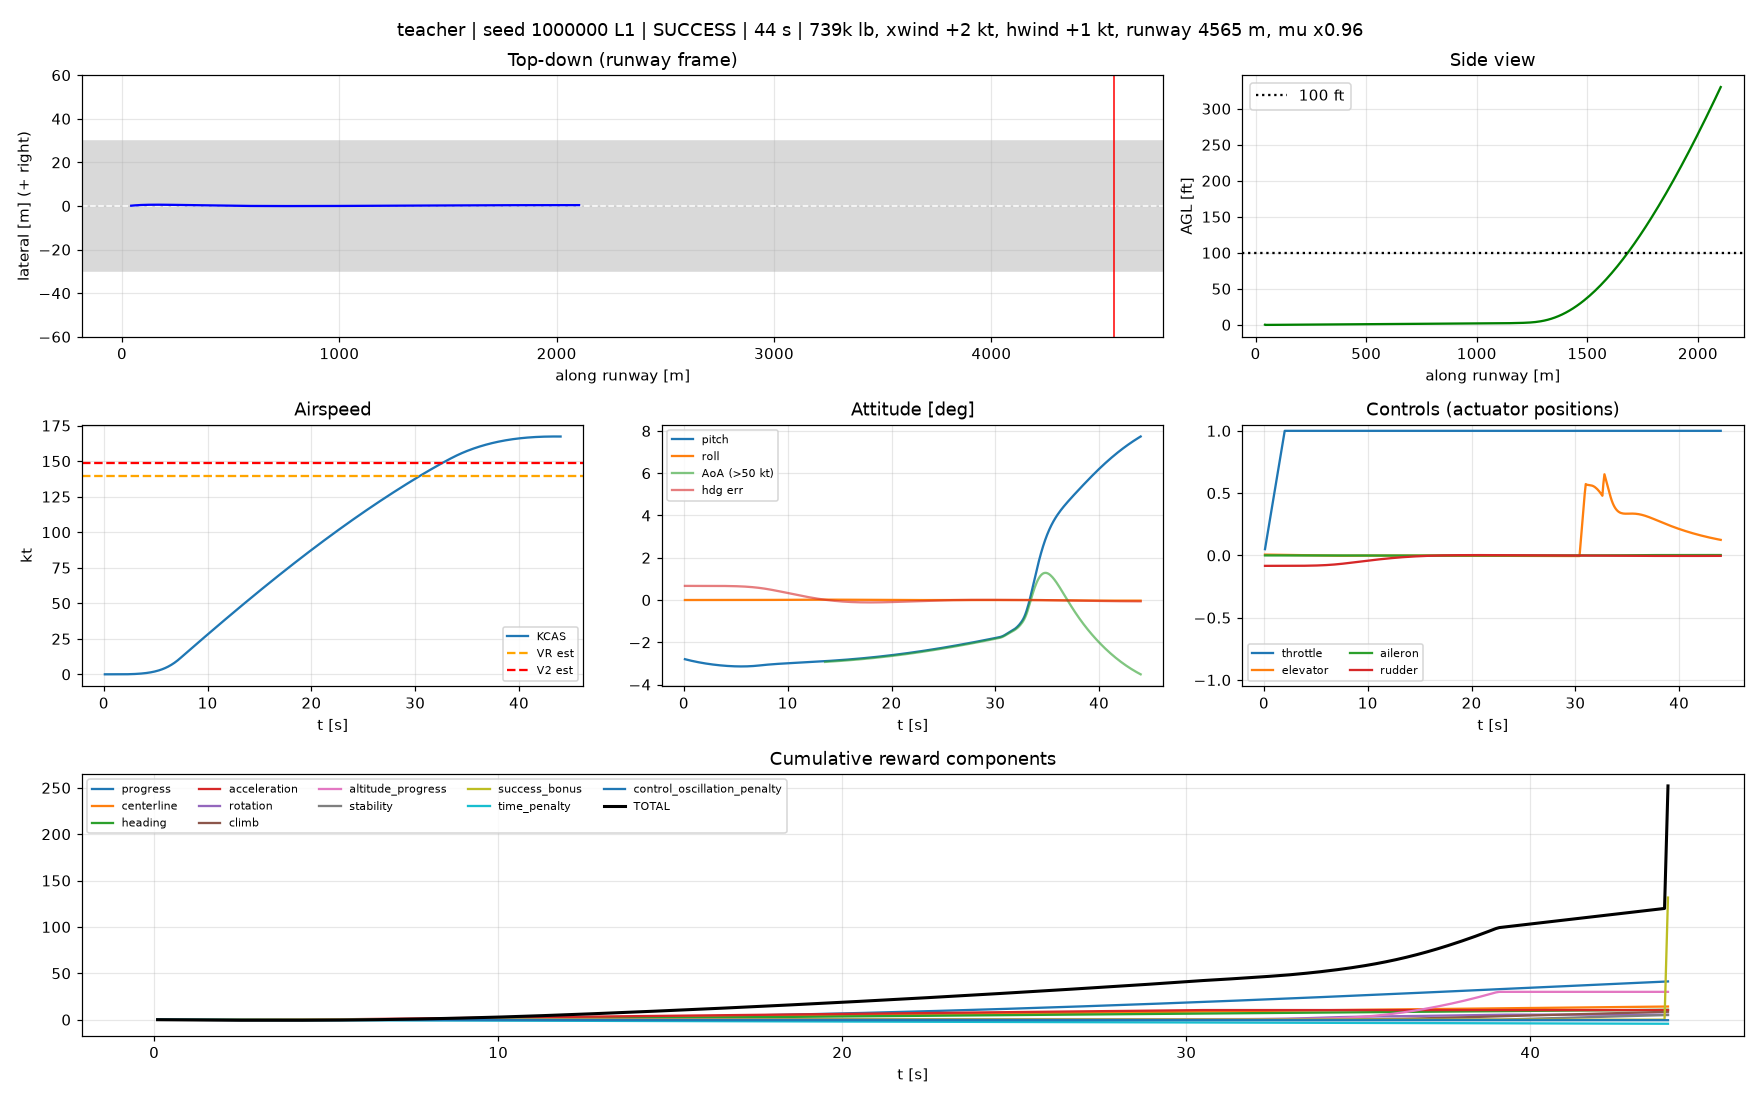
\includegraphics[width=0.96\linewidth]{../assets/teacher_success_dashboard.png}\caption{SUCCESS: the teacher's centerline error stays small, speed rises, and height climbs. The control traces are comparatively calm.}\end{figure}
Read the top-down trace first: it stays near the runway middle. Read airspeed next: it rises to rotation. Then read height and climb: they continue upward. Finally check pitch, roll and controls: no large oscillation is needed. This dashboard records an actual successful teacher simulation, not a hypothetical example.

\begin{figure}[htbp]\centering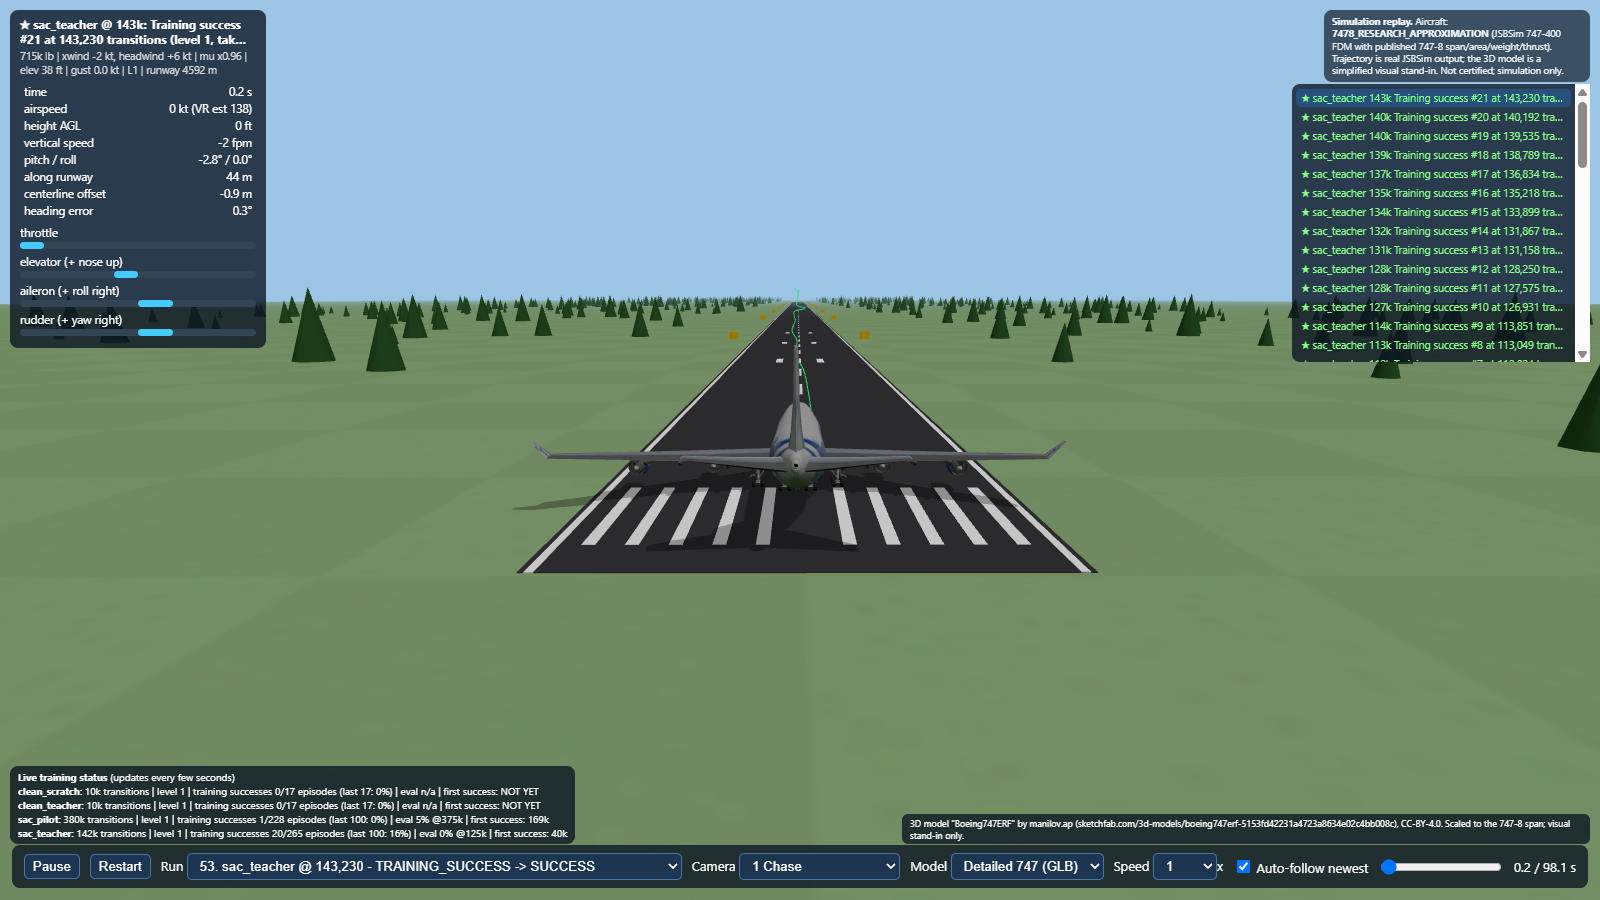
\includegraphics[width=0.96\linewidth]{../assets/training_success_3d.png}\caption{SUCCESS IN 3D: a recorded training-success replay; the event list contains multiple real successful episodes.}\end{figure}
\begin{figure}[htbp]\centering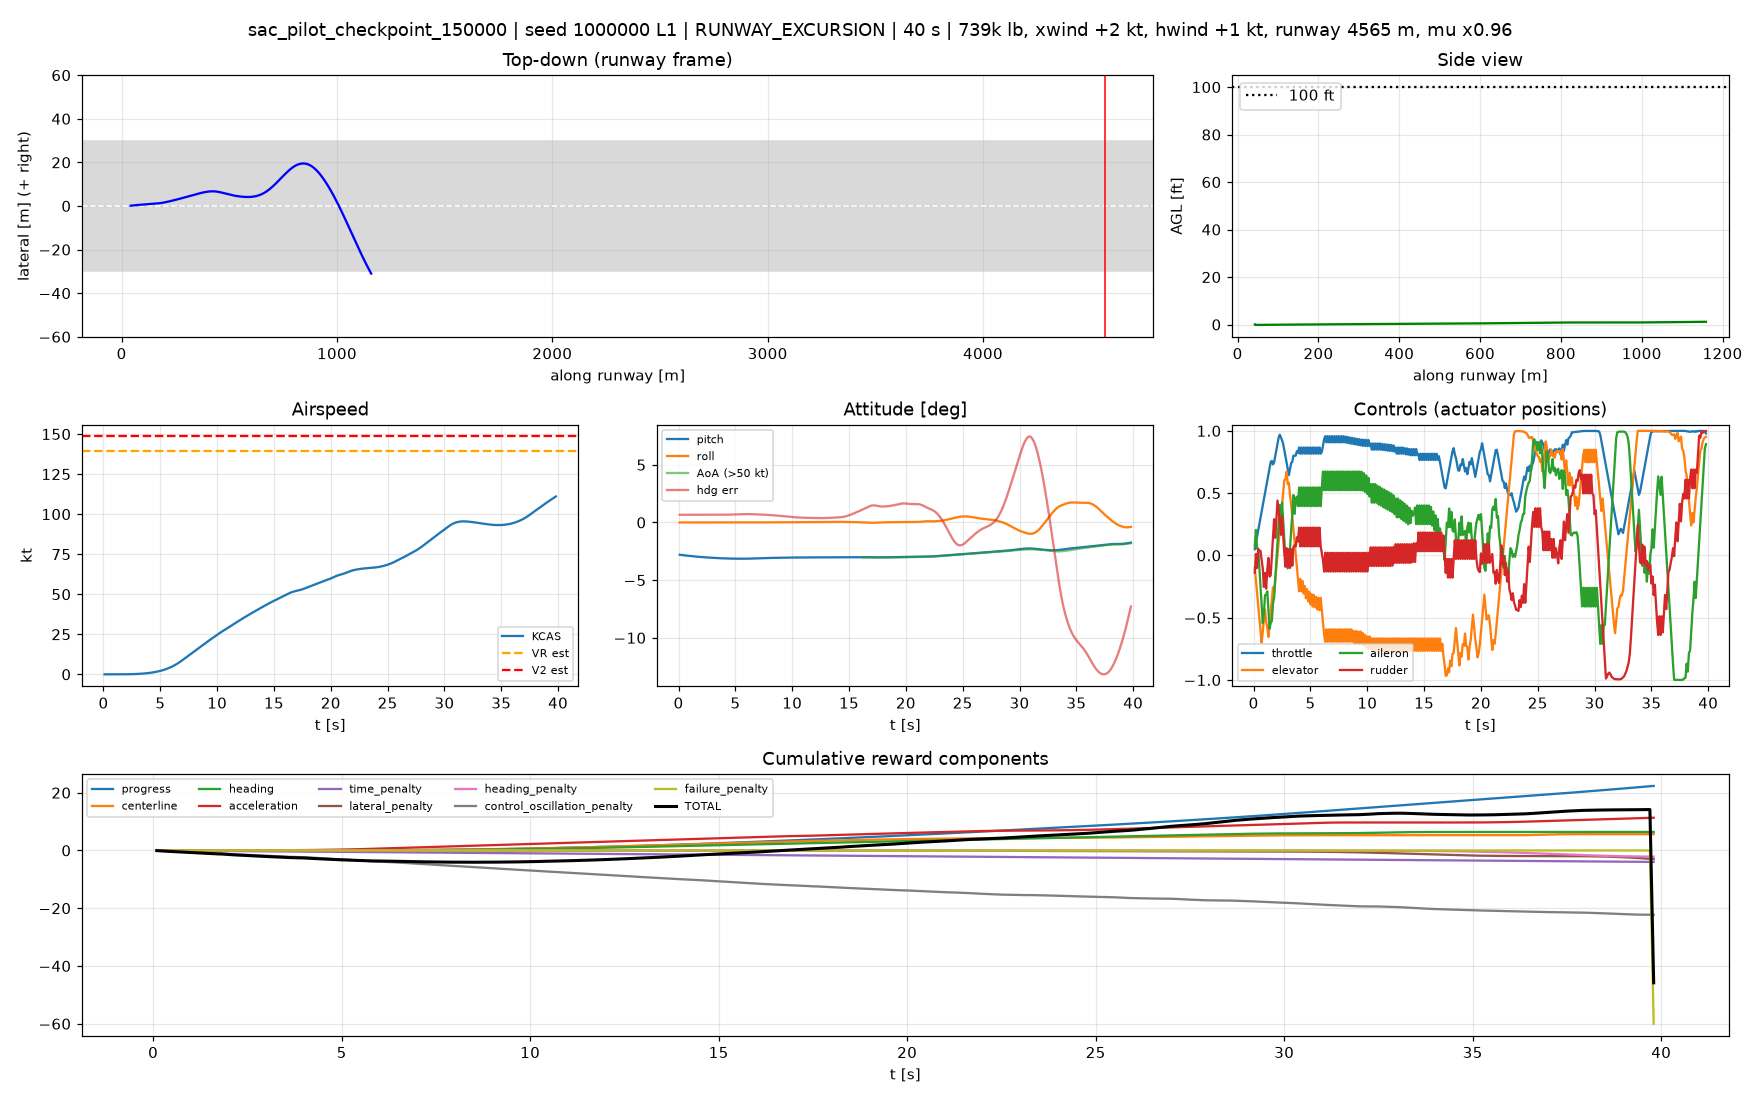
\includegraphics[width=0.96\linewidth]{../assets/early_agent_failure.png}\caption{FAILURE: an early SAC policy wanders off the runway; the controls swing rapidly and the altitude does not show a successful climb.}\end{figure}
On the failure dashboard, centerline error grows instead of shrinking and control traces become jagged. The right response is to inspect action signs, rate limits, lateral reward components and the observation values on that trajectory. A failure image is a debugging clue, not proof that the whole algorithm is broken.

\section{How to rebuild from an empty folder}
A clean rebuild needs Python 3.10-3.13, Git, the dependencies in requirements.txt, and a terminal. The project uses a Python virtual environment to keep packages separate. On Windows PowerShell, the following is the shortest reproducible path.

\begin{Verbatim}[fontsize=\small]
git clone https://github.com/malekawlaqi/Autonomous-airplane-project.git
cd Autonomous-airplane-project\boeing7478_rl_takeoff
python -m venv .venv
.venv\Scripts\python.exe -m pip install -r requirements.txt
.venv\Scripts\python.exe tools\inspect_aircraft.py
.venv\Scripts\python.exe tools\check_environment.py
.venv\Scripts\python.exe -m pytest
\end{Verbatim}
The clone command needs access to the private GitHub repository. If PyTorch GPU support is desired, follow the project's README for the compatible CUDA wheel; CPU mode works for setup checks but training speed can differ. Run commands from the boeing7478\_rl\_takeoff directory so relative config and output paths resolve correctly.

To reimplement the *software* from scratch rather than clone it, build in this order: (1) YAML configs and an honest aircraft-model note, (2) JSBSim adapter with verified sensor/control properties, (3) runway frame and seeded randomizer, (4) observation builder, (5) action mapper, (6) success/failure tracker, (7) reward components, (8) Gymnasium reset/step, (9) teacher and baselines, (10) environment tests, (11) SAC driver, (12) evaluation/curriculum/checkpoint callbacks, and (13) replay/report tools. Validate each small layer before adding the next.

\begin{longtable}{|p{0.47\linewidth}|p{0.47\linewidth}|}\hline
Build milestone & Small proof before moving on \\ \hline
Simulator adapter & Load model; read every required property; step physics without NaN. \\ \hline
Runway geometry & Forward distance increases; right-side error has the expected sign. \\ \hline
Actions & Measured nose/roll/yaw move in the documented positive directions. \\ \hline
Gym environment & Reset gives 27 finite values; step gives a bounded observation and four controls. \\ \hline
Teacher & At least one valid takeoff under easy conditions. \\ \hline
SAC & Checkpoint, evaluate, interrupt and resume all work. \\ \hline
Generalization & Compare several fixed seeds and harder levels to teacher and full-throttle baselines. \\ \hline
\end{longtable}
\section{First hands-on experiment}
Begin by watching the teacher and a simple full-throttle baseline. This confirms whether the environment is solvable and shows that takeoff alone does not prove learning. Then generate teacher demonstrations, train a *new* SAC run, inspect the CSV and replay. Avoid reusing the active run name if the original trainer is still writing to it.

\begin{Verbatim}[fontsize=\small]
.venv\Scripts\python.exe -m evaluation.evaluate --policy teacher --episodes 20 --level 1
.venv\Scripts\python.exe -m evaluation.evaluate --policy full_throttle --episodes 20 --level 1
.venv\Scripts\python.exe -m teacher.demonstrations --episodes 200 --level 1 --out results/demos/teacher_demos.npz
.venv\Scripts\python.exe -m training.train_sac --config configs/sac.yaml --run-name beginner_rebuild --demos results/demos/teacher_demos.npz --bc-epochs 20 --total-timesteps 500000
\end{Verbatim}
A training transition is one action plus 12 physics steps, about 0.1 simulated seconds. A 50-second episode is roughly 500 transitions. The 500,000-transition target is therefore many whole attempts, not 500,000 rendered video frames. Training uses headless physics for speed; 3D replay records trajectories later.

\section{How to judge whether learning is real}
Use deterministic evaluation with fixed seeds separate from training. Report success rate and its episode count, takeoff time, runway distance, centerline RMS/max error, cleanliness and failure reasons. Compare with the teacher and full-throttle baseline on the same difficulty. Repeat the training with at least three training seeds before claiming one method is better. A 20-episode result is a progress signal, not a final confidence estimate.

The reward can be gamed. A policy might earn progress points while staying unsafe, or look good on level 1 while failing in crosswind. That is why the project has separate terminal success rules, comfort metrics, baseline policies, held-out evaluation seeds and robustness tests. A curriculum level-up may cause the displayed success rate to drop because the exam became harder.

\begin{figure}[htbp]\centering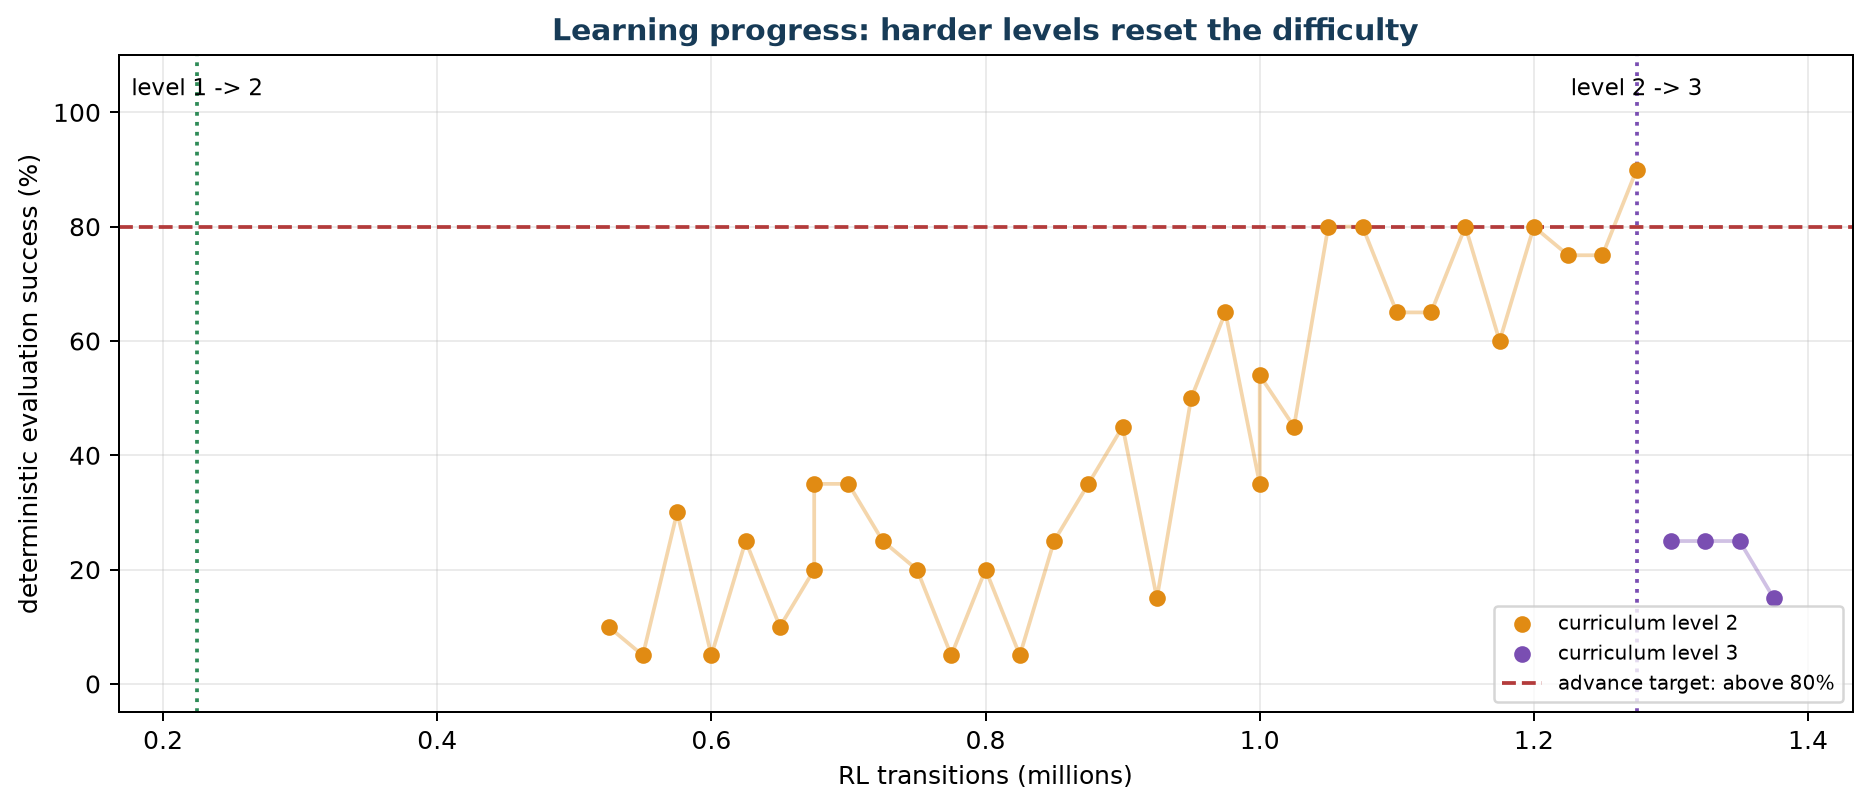
\includegraphics[width=0.96\linewidth]{../assets/evaluation_progress.png}\caption{Evaluation success over transitions. Interpret each point together with its curriculum level and episode count.}\end{figure}
\section{Where this project stands today}
The included report snapshot was captured at 2026-10-08 11:34 Maroc. The named run was clean\_teacher\_lv4, with 1,386,000 transitions, 920 training episodes and 585 training successes. It was on curriculum level 3. The latest 100 training episodes had 42\% success; the latest deterministic level-3 evaluation had 15\% success over 20 episodes. The first successful training episode occurred at 107,676 transitions. Training may have continued after this snapshot.

What this means: the system learned complete takeoffs at easier levels and has reached level 3, but level-3 reliability is still low. The next developer should diagnose level-3 outcomes, especially unclean takeoffs and insufficient acceleration, with fixed-seed comparisons. The repository is a research prototype, not a finished robust pilot.

\begin{figure}[htbp]\centering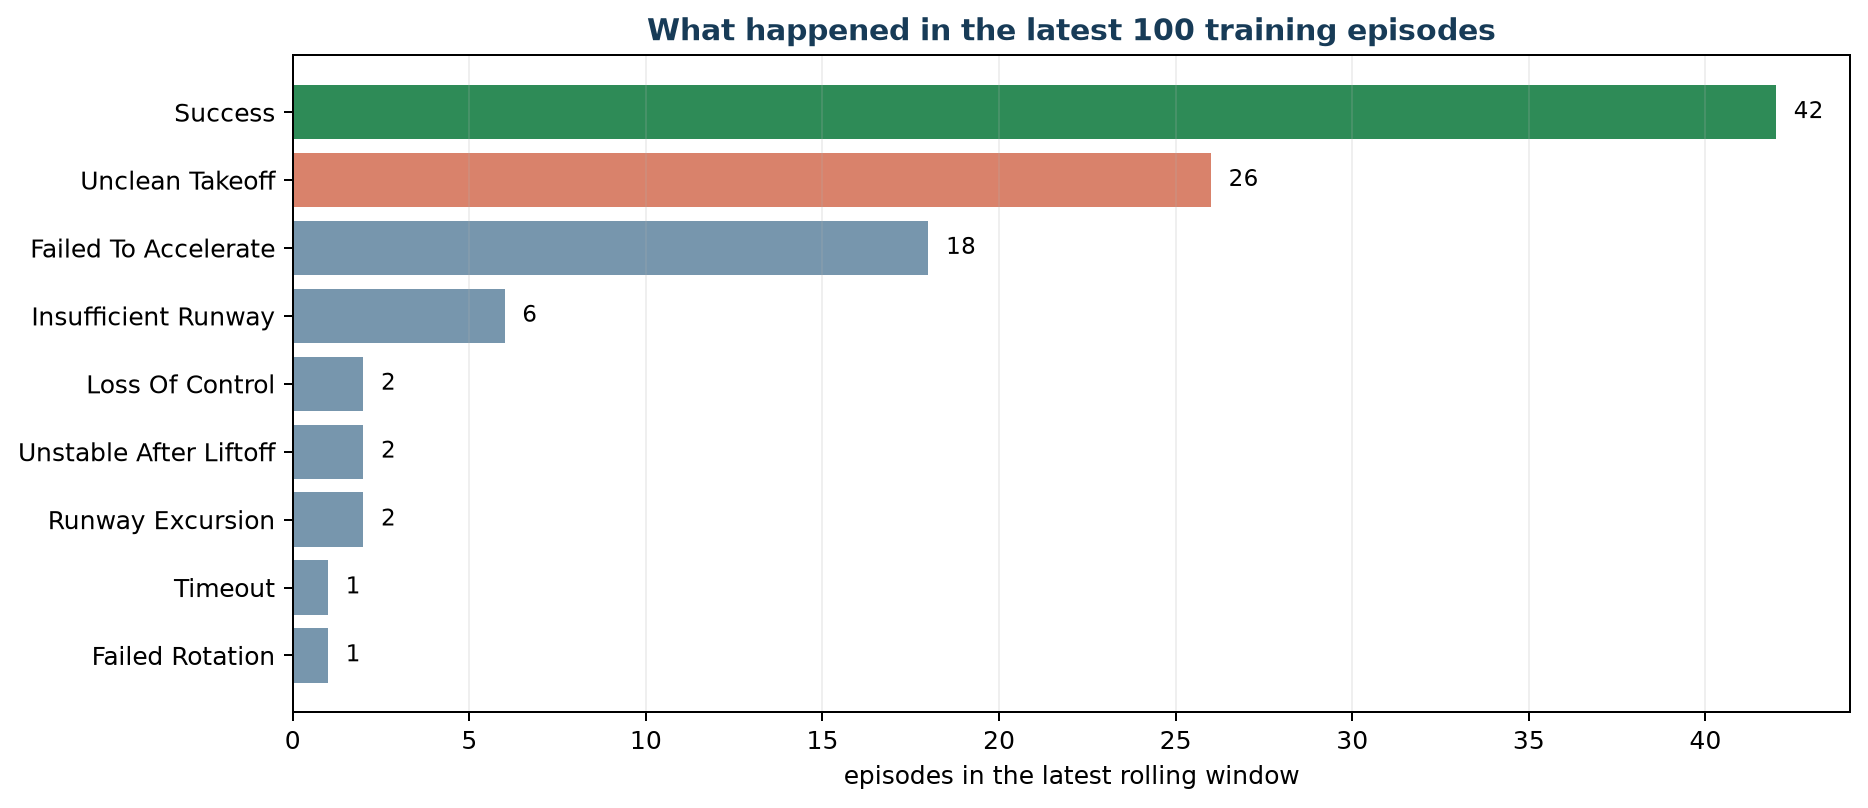
\includegraphics[width=0.96\linewidth]{../assets/recent_outcomes.png}\caption{A snapshot of recent outcomes. Look beyond the total success count and inspect each failure category.}\end{figure}
\section{Practical continuation and common questions}
\begin{longtable}{|p{0.47\linewidth}|p{0.47\linewidth}|}\hline
Question & Answer \\ \hline
Where do I start reading? & README, this guide, aircraft notes, then envs/boeing7478\_takeoff\_env.py. \\ \hline
What if check\_environment fails? & Inspect the named check; verify JSBSim, config files and aircraft property names before training. \\ \hline
Why does GPU use look low? & JSBSim physics is CPU-bound; the GPU only helps neural-network updates. \\ \hline
Why does the viewer differ from training? & Viewer uses a visual 747 model; flight physics comes from the JSBSim approximation. \\ \hline
Why can a neutral controller take off? & The inherited model is forgiving; compare centerline, comfort and robustness, not lift-off alone. \\ \hline
Why is success lower after level-up? & New evaluation conditions are harder. Read level and seed alongside rate. \\ \hline
Can I change reward weights and resume? & Use a new run name/profile; a changed reward defines a different learning problem. \\ \hline
What is missing from GitHub? & Virtual environments, logs, temp files and huge replay buffers; recreate or copy them separately. \\ \hline
What makes a resume exact? & Matching model zip, replay-buffer pickle, state JSON, config and reward profile. \\ \hline
Can this control a real aircraft? & No. The model is unvalidated and this is simulation research only. \\ \hline
\end{longtable}
Next-work checklist: read the newest results; preserve the active trainer's files; run checks when the trainer is paused; evaluate the current checkpoint on a fixed set of level-3 seeds; count failure reasons; replay representative successes and failures; change one hypothesis at a time; test against teacher/full-throttle baselines; repeat over multiple training seeds; update the results table and report with dated measurements.

\section{Source map and reading order}
This guide was checked against the repository files listed below. Follow the order for a code review: configuration and aircraft notes -> environment reset/step -> observation/action helpers -> termination/reward -> teacher -> SAC driver -> callbacks -> evaluation -> tests -> result CSVs. A source line number is a signpost for learning, not a promise that future commits keep the same numbering.

\begin{longtable}{|p{0.47\linewidth}|p{0.47\linewidth}|}\hline
Source & Purpose \\ \hline
README.md; AIRCRAFT\_MODEL\_NOTES.md; EXPERIMENT\_PROTOCOL.md & Scope, caveats, commands and experiment rules. \\ \hline
configs/*.yaml & Physics rate, success limits, reward weights, aircraft overrides, SAC settings and randomization. \\ \hline
envs/*.py & The Gymnasium task, JSBSim bridge, runway math, sensors, actions, reward and outcomes. \\ \hline
teacher/*.py & Simple controller, demonstration collection and behavior cloning. \\ \hline
training/*.py & SAC training, curriculum, logging, evaluation and checkpointing. \\ \hline
evaluation/*.py & Policy exams, robustness, failure tables and replay trajectories. \\ \hline
tests/*.py; tools/check\_environment.py & Automated checks of shapes, signs, reward arithmetic and episode behavior. \\ \hline
results/replay/*.png; results/replay3d/*.png & The actual success/failure visual evidence used here. \\ \hline
\end{longtable}
The UM6P College of Computing and Forgebots marks on the cover were extracted from the existing club report in this repository, so this handbook uses the same visual identity.

\section{Reimplementation acceptance checklist}
A rebuild is complete only when another person can run the same checks and explain the results. Use this short checklist as the last page of the handover.

\begin{longtable}{|p{0.47\linewidth}|p{0.47\linewidth}|}\hline
Check & Expected evidence \\ \hline
Aircraft identity & The inspector prints 7478\_RESEARCH\_APPROXIMATION and names the generated model. \\ \hline
Gymnasium interface & reset returns 27 finite values; step returns observation, reward, terminated, truncated and info. \\ \hline
Control directions & Positive nose-up, right-roll and right-yaw agent commands move the simulator in the documented directions. \\ \hline
Reproducible weather & A fixed seed gives the same episode conditions and a changed seed gives a different draw. \\ \hline
Teacher and baselines & The teacher reaches at least one valid takeoff; full-throttle baseline is measured too. \\ \hline
Training recovery & A checkpoint saves model zip, state JSON and local replay buffer; interruption and resume are tested. \\ \hline
Honest evaluation & Fixed unseen seeds produce a success rate, episode count, failure table and comfort metrics. \\ \hline
\end{longtable}
If a check fails, stop at that layer and repair it before a long training run. This prevents a neural network from learning around a simulator bug. Keep the 3D viewer as a way to understand recorded flights, while using the numeric evaluator as the source of performance claims.

\end{document}